\section{Introduction}
\label{sec:introduction}

\ac{HPC} systems increasingly handle massive, resource-intensive tasks that demand significant memory capacity for storage, intermediate computations, and output generation.
Seismic workloads exemplify this challenge, with input volumes often spanning hundreds of gigabytes and numerical methods introducing additional complexity through temporary buffers, matrix operations on large arrays, and partial result storage.

Distributed platforms such as Dask~\cite{rocklin2015dask} address these challenges by facilitating horizontal scaling, enabling multiple workers to process data segments (chunks) in parallel.
This concurrency substantially reduces execution time but introduces critical risks when resource demands are underestimated.
Dask's default chunking heuristics distribute data based on file-block boundaries or user-defined size targets without considering operator-specific memory requirements or data types.

\subsection{The Chunking Challenge}

The selection of appropriate chunk sizes is fundamental to efficient data-parallel processing.
As illustrated in Figure~\ref{fig:chunking-example}, chunk configurations can vary widely, and naive choices lead to suboptimal performance.
Overfragmented approaches with many small chunks incur excessive task scheduling overhead and poor computational efficiency, while oversized chunks can exceed available memory capacity and trigger \ac{OOM} errors.

\subsubsection{Memory Consumption Patterns}

Understanding memory consumption patterns in scientific computing workloads is crucial for effective chunking.
Our analysis of seismic processing operators reveals several key characteristics:

\begin{itemize}
    \item \textbf{Linear scaling}: Memory usage typically scales linearly with input volume for tensor operations
    \item \textbf{Operator-specific constants}: Different algorithms have varying memory multiplication factors
    \item \textbf{Intermediate expansions}: Many operations create temporary arrays 2-10× the input size
    \item \textbf{Framework overhead}: Distributed computing frameworks add 10-20\% memory overhead
\end{itemize}

These patterns make manual chunk size selection particularly challenging, as users must account for both the base memory requirements and dynamic expansions during computation.

\subsubsection{Current Practice Limitations}

Existing approaches to chunk size selection suffer from several limitations:

\begin{enumerate}
    \item \textbf{Trial-and-error}: Users iteratively adjust chunk sizes until finding a configuration that avoids \ac{OOM} errors, wasting computational resources on failed attempts
    \item \textbf{Conservative overprovisioning}: To avoid failures, users often select very small chunks, leading to excessive fragmentation and poor performance
    \item \textbf{Static heuristics}: Fixed rules like "128MB per chunk" fail to account for operator-specific memory patterns
    \item \textbf{Lack of adaptation}: Current methods cannot adjust to different algorithms or data characteristics
\end{enumerate}

\begin{figure}[ht]
    \centering
    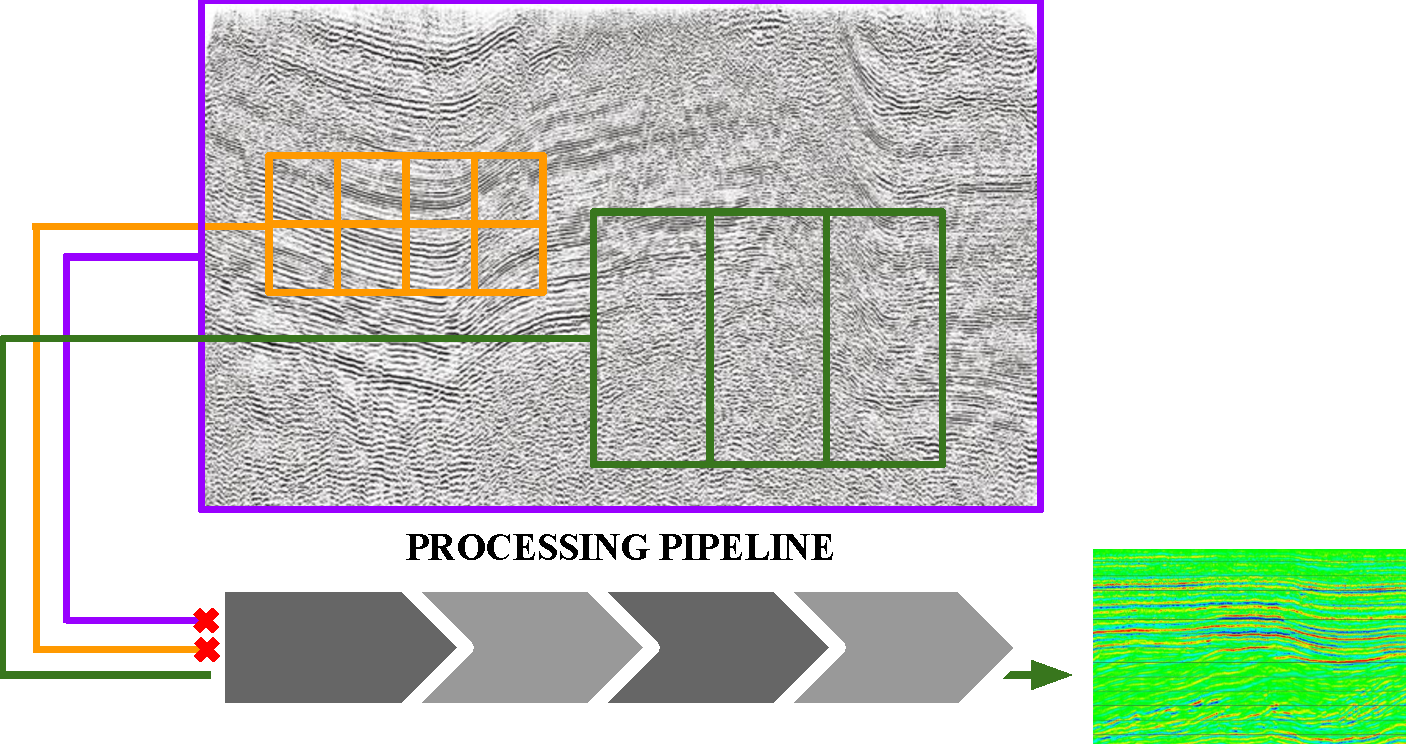
\includegraphics[width=0.7\textwidth]{assets/images/chunking-example}
    \caption{Seismic data chunking strategies.
    The purple rectangle shows the entire volume, orange rectangles represent overfragmented chunking (red × marks indicate failure), and green rectangles show balanced chunking that better utilizes resources.}
    \label{fig:chunking-example}
\end{figure}

In memory-intensive computations, particularly seismic processing with convolution-based algorithms or 3D filtering, unpredictable memory spikes from short-lived but large intermediate arrays make robust memory-aware chunk sizing essential.
Current practice relies on heuristic tuning or trial-and-error approaches, where operators execute multiple iterations with various chunk configurations searching for optimal partitioning.
This methodology is computationally expensive and inefficient, as unsuccessful trials consume significant resources without producing beneficial outcomes.

\subsection{Contributions}

This paper presents a novel memory-aware chunking mechanism that addresses these limitations by employing predictive modeling to anticipate memory consumption based on input data shapes and operator characteristics.
Our key contributions include:

\begin{enumerate}
    \item A systematic approach to predict memory requirements for tensor-based operations using regression models trained on profiling data
    \item An automated chunk sizing algorithm that ensures memory usage remains within specified thresholds while maximizing computational efficiency
    \item Comprehensive experimental evaluation demonstrating elimination of \ac{OOM} errors and competitive performance compared to existing heuristic methods
    \item Integration with Dask's distributed computing framework, providing a practical solution for production \ac{HPC} environments
\end{enumerate}

The remainder of this paper is organized as follows: Section~\ref{sec:related-work} reviews related work in memory management and chunking strategies.
Section~\ref{sec:methodology} details our memory-aware chunking approach.
Section~\ref{sec:experimental-results} presents experimental evaluation across various workloads and configurations.
Finally, Section~\ref{sec:conclusion} summarizes findings and discusses future directions.